

\chapter{The \bitstream Layer}

Conceptually, a \emph{bit stream}~$b$ is a sequence~$b_0,\ldots,b_{n-1}$ of $n$~bits.
Since the \isoc programming language does not allow to directly declare bit sequences
we represent bit streams as \emph{byte arrays}, that is, as arrays of type \inl{uint8_t}
(see Figure~\ref{fig:byte-array}).

\begin{figure}[hbt]
\begin{center}
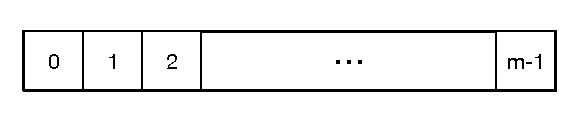
\includegraphics[scale=0.99]{Figures/byte-array.pdf}
\caption{Indexing in a byte array}
\label{fig:byte-array}
\end{center}
\end{figure}

If $x$ is a value of type \inl{uint8_t}, then its uniquely determined binary representation 
\begin{align*}
   x &= \sum_{i = 0}^{7} x_i\cdot 2^i && \text{with } x_k \in \{0, 1\} \text{ for } 0 \leq k < 8
\intertext{suggests an ordering of the bits of $x$ \emph{from the right}, that is, starting with the
position~0 of the \emph{least significant bit} of $x$}
   x &= (x_7,x_6,x_5,x_4,x_3,x_2,x_1,x_0)
\end{align*}

The ETCS standard, however, mandates that numerical values shall be transmitted
starting from the \emph{most significant bit}.
We therefore use the scheme of Figure~\ref{fig:bit-stream} for indexing bits within a byte stream.

\begin{figure}[hbt]
\begin{center}
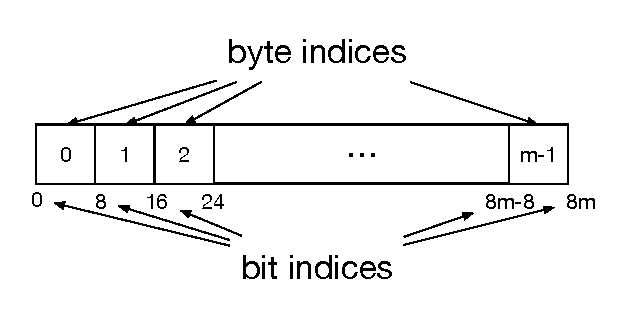
\includegraphics[scale=0.89]{Figures/bit-stream.pdf}
\caption{Indexing in a bit stream}
\label{fig:bit-stream}
\end{center}
\end{figure}

\section{The Type \bitstream and Related Functions}

The type \bitstream in Listing~\ref{lst:bitstream} is our \isoc representation of a bit stream.


\begin{listing}[hbt]
\begin{center}
\begin{lstlisting}[style=acsl-block]
struct Bitstream
{
    uint8_t*  addr;
    uint32_t  size;
    uint32_t  bitpos;
};

typedef struct Bitstream Bitstream;
\end{lstlisting}
\end{center}
\caption{\label{lst:bitstream} Definition of type \bitstream}
\end{listing}

Figure~\ref{fig:bit-stream-type}  shows that for an object of type \bitstream the field \inl{addr} is the
starting address of a byte array of \inl{size} elements and that the field \inl{bitpos}
denotes a bit position within this byte array.

\begin{figure}[hbt]
\begin{center}
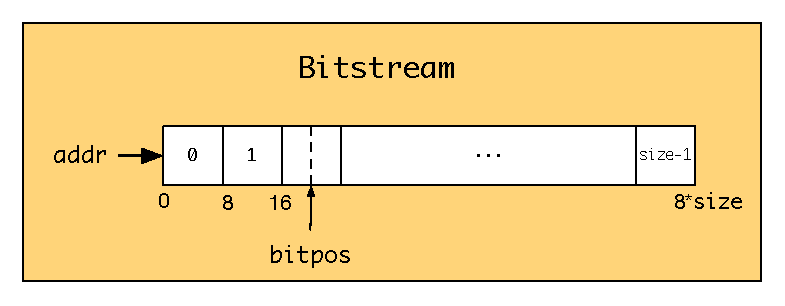
\includegraphics[scale=0.85]{Figures/bit-stream-type.pdf}
\caption{The type \bitstream}
\label{fig:bit-stream-type}
\end{center}
\end{figure}

An obvious type invariant of \bitstream is the condition
\begin{align}
\label{eq:bit-stream-invariant}
    0 \leq \mathtt{bitpos} < 8 \cdot \mathtt{size}
\end{align}

\clearpage

\subsection{The Function \bitstreamread}

The function \bitstreamread, whose declaration is shown in Listing~\ref{lst:bitstream-read-declaration}
reads a sequence of bits from a bit stream and copies the bits into a value of \inl{uint64_t}.


\begin{listing}[hbt]
\begin{lstlisting}[style=acsl-block]
    uint64_t Bitstream_Read(Bitstream* stream, uint32_t length);
\end{lstlisting}
\caption{\label{lst:bitstream-read-declaration} Declaration of \bitstreamread}
\end{listing}

\FloatBarrier

The informal semantics of \bitstreamread is depicted in Figure~\ref{fig:bit-stream-read}.

\begin{figure}[hbt]
\begin{center}
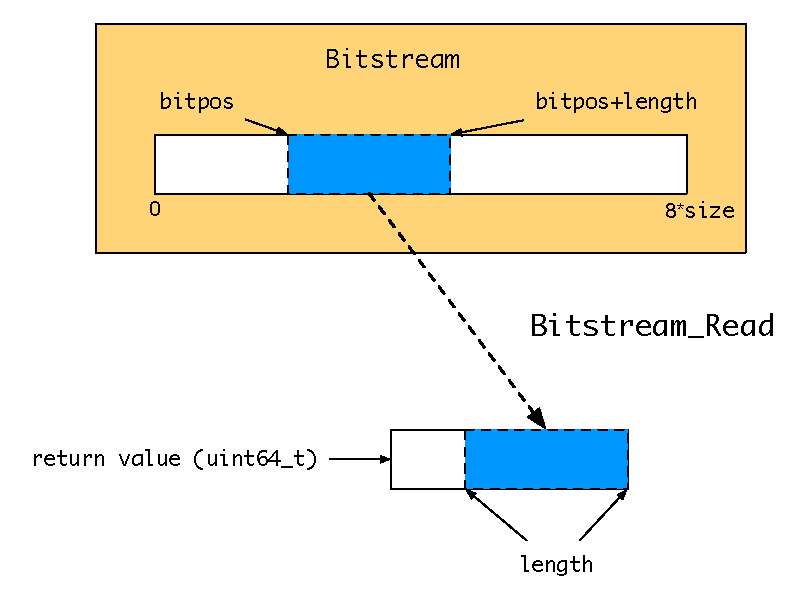
\includegraphics[scale=0.85]{Figures/bit-stream-read.pdf}
\caption{Informal description of \bitstreamread}
\label{fig:bit-stream-read}
\end{center}
\end{figure}

Figure~\ref{fig:bit-stream-read} also suggests the following preconditions of \bitstreamread
\begin{subequations}
\label{eq:bit-stream-read-pre}
\begin{align}
   \mathtt{length} &\leq 64 \\
   \mathtt{bitpos} + \mathtt{length} &\leq 8 \cdot \mathtt{size}
\end{align}
\end{subequations}

\clearpage

\subsection{The Function \bitstreamwrite}

The Function \bitstreamwrite (see Listing~\ref{lst:bitstream-write-declaration})
is, in simple terms, the inverse of \bitstreamread.
It takes \inl{length} bits of the argument \inl{value} and writes it into the bit stream.

\begin{listing}[hbt]
\begin{lstlisting}[style=acsl-block]
    void Bitstream_Write(Bitstream* stream, uint32_t length, 
                         uint64_t value);
\end{lstlisting}
\caption{\label{lst:bitstream-write-declaration} Declaration of \bitstreamwrite}
\end{listing}

The informal semantics of \bitstreamwrite is depicted in Figure~\ref{fig:bit-stream-write}.

\begin{figure}[hbt]
\begin{center}
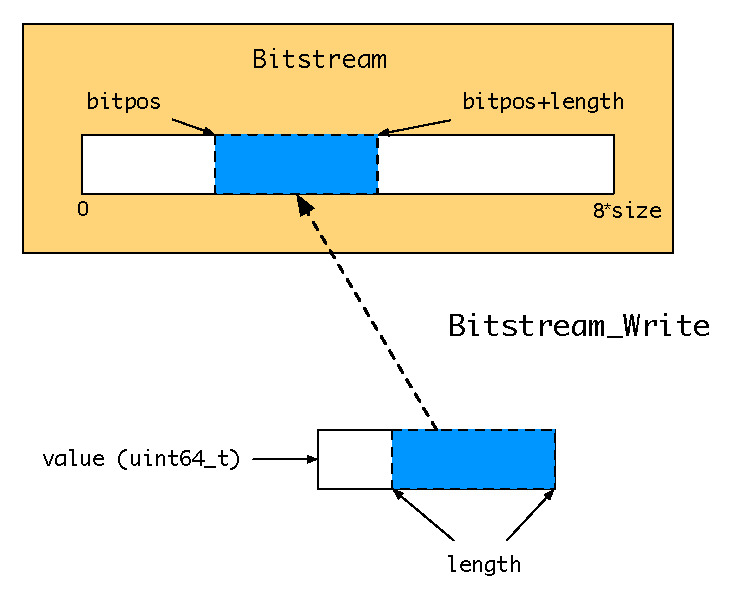
\includegraphics[scale=0.85]{Figures/bit-stream-write.pdf}
\caption{Informal description of \bitstreamwrite}
\label{fig:bit-stream-write}
\end{center}
\end{figure}

In addition to the preconditions~\eqref{eq:bit-stream-read-pre} one must ensure
that the argument \inl{value} can be represented by \inl{length} bits.
In other words, the following precondition must also be satisfied.

\begin{align}
\label{eq:bit-stream-write-pre}
    \mathtt{value} < 2^{\mathtt{length}}
\end{align}

\subsection{The Function \inl{NormalBitstream}}

\fxfatal{does this function belong to the public interface?}

\section{Predicates}

In this section we define several \acsl predicates that will be of use when
formally specifiying the functions \bitstreamread and \bitstreamwrite.


\subsection{The Predicates \readable and \writeable}

Listing~\ref{lst:readable-writeable} shows the two predicates \readable and \writeable.

\begin{listing}[hbt]
\begin{lstlisting}[style=acsl-block]
/*@
  predicate 
    Readable{L}(Bitstream* stream) =
        \valid(stream) &&
        \valid_read(stream->addr + (0..stream->size-1));

  predicate
    Writeable{L}(Bitstream* stream) =
        \valid(stream) &&
        \valid(stream->addr + (0..stream->size-1));
*/
\end{lstlisting}
\caption{\label{lst:readable-writeable} The predicates \readable and \writeable}
\end{listing}

Both predicates in Listing~\ref{lst:readable-writeable}
take as argument a valid pointer to \bitstream.
They differ only in the fact that in the case of \readable
the array \inl{addr[0..size-1]} is only declared as \emph{valid for reading}.
In the case of \writeable this array is generally valid, that is, both for reading and writing.

\subsection{The Predicates \invariant and \normal}

\begin{listing}[hbt]
\begin{lstlisting}[style=acsl-block]
/*@
  predicate 
    Invariant{L}(Bitstream* stream, integer length) =
        \separated(stream, stream->addr + (0..stream->size-1)) &&
        BitwalkerInvariant{L}(stream->size, stream->bitpos, length);

  predicate
    Normal{L}(Bitstream* stream, integer length) =
      NormalBitwalker(stream->size, stream->bitpos, length);
*/
\end{lstlisting}
\caption{\label{lst:invariant-normal} The predicates \invariant and \normal}
\end{listing}

\clearpage

\subsection{The Predicates \equalbits and \unchanged}

\begin{listing}[hbt]
\begin{lstlisting}[style=acsl-block]
/*@
  predicate
   EqualBits{A}(Bitstream* stream, integer first, integer last, uint64_t value) =
      EqualBits{A}(stream->addr, first, last, value);

  predicate
    Unchanged{A,B}(Bitstream* stream, integer first, integer last) =
     \forall integer i;  first <= i < last ==>
        (LeftInBitstream{A}(stream, i) <==> LeftInBitstream{B}(stream, i));
\end{lstlisting}
\caption{\label{lst:equalbits-unchanged} The predicates \equalbits and \unchanged}
\end{listing}


\subsection{The Predicate \upperbitsnotset}

\begin{listing}[hbt]
\begin{lstlisting}[style=acsl-block]
/*@
   predicate
     UpperBitsNotSet{A}(integer value, integer length) =
       \forall integer i; length <= i ==> !BitTest(value, i);
\end{lstlisting}
\caption{\label{lst:upperbitsnotset} The predicate \upperbitsnotset}
\end{listing}

\section{Formal Specification}
\subsection{The Function \bitstreamread}
\subsection{The Function \inl{Bitstream_Write}}
\subsection{The Function \inl{NormalBitstream}}

\section{Implementation}
\subsection{The Function \bitstreamread}
\subsection{The Function \inl{Bitstream_Write}}
\subsection{The Function \inl{NormalBitstream}}

\section{Formal Verification}
\subsection{\inl{Bitstream_ReadThenWrite}}
\subsection{\inl{Bitstream_WriteThenRead}}

